\documentclass[aspectratio=1610, 13pt]{beamer}
\usepackage{xcolor}
\usepackage{multicol}
\usepackage{mathtools,array}
\usepackage[T1]{fontenc}

\usepackage{dutchcal}
\usepackage{zi4}
\usepackage[font={scriptsize,bf}]{caption}
% \usepackage{subcaption}
\usepackage{graphics}
\usepackage{tikz}
\usepackage{fontawesome5}
\usepackage{mathpartir}

\newcommand{\naturals}{\mathbb{N}}
\newcommand{\reals}{\mathbb{R}}

\newcommand{\Dist}[1]{\mathcal{D}(#1)}
\newcommand{\expectation}{\mathbb{E}}

\newcommand{\states}{S}
\newcommand{\actions}{A}
\newcommand{\observables}{O}
\newcommand{\trans}{T}
\newcommand{\obs}{Z}
\newcommand{\reward}{R}
\newcommand{\discount}{\gamma}

\newcommand{\beliefs}{\mathcal{B}}
\newcommand{\beliefUpdate}{\tau}

\newcommand{\policy}{\pi}

\newcommand{\diff}[1]{\mathop{}\!\mathrm{d}#1}
\renewcommand{\figurename}{Figure}
\renewcommand{\refname}{Reference}

\AtBeginDocument{
  \catcode`_=12
  \begingroup\lccode`~=`_
  \lowercase{\endgroup\let~}\sb
  \mathcode`_="8000
}

% \usetheme{Madrid}
% % \usetheme{default}
% \setbeamertemplate{caption}[numbered]
% \setbeamerfont{title}{size=\large}
\mode<presentation>
{
  \usetheme{Darmstadt}      % or try Darmstadt, Madrid, Warsaw, ...
  \usecolortheme{default} % or try albatross, beaver, crane, ...
  \usefonttheme[onlymath]{serif}  % or try serif, structurebold, ...
  \setbeamertemplate{navigation symbols}{}
  \setbeamertemplate{caption}[numbered]
  \setbeamertemplate{footline}[frame number] 
} 

\usepackage{listings}
\lstdefinestyle{heaplang}{
    language=Caml,
    basicstyle=\footnotesize\ttfamily,
    keywordstyle=\color{blue},
    commentstyle=\color{red},
    escapeinside={<@}{@>},
    morekeywords={new_chan, fork, recv, send, swap, ref}
}
\lstdefinestyle{clang}{
    language=Caml,
    basicstyle=\footnotesize\ttfamily,
    keywordstyle=\color{blue},
    commentstyle=\color{red},
    escapeinside={<@}{@>},
}
\lstset{style=heaplang}

\usepackage{natbib}

\newcommand{\buchi}{B\"uchi }

\definecolor{goldenpoppy}{rgb}{0.99, 0.76, 0.0}
\definecolor{goldenyellow}{rgb}{1.0, 0.87, 0.0}
\definecolor{green2}{rgb}{0.1,0.7,0.3} 
\newcommand{\gcheck}{{\color{green2}\faCheckCircle[regular] }}
\newcommand{\rcross}{{\color{red} \faTimesCircle[regular]} }
\newcommand{\rflag}{{\color{red} \faFlag}}
% \usepackage{algorithm,amsmath}
% \usepackage[noend]{algpseudocode}

\newcommand{\zlstinline}{\let\par\endgraf\lstinline}
\newcommand{\comments}[1]{{\color{red}#1}}
\title{Section 2.6 Shape Analysis}
\author{Reporter:  Xie Li}
\date{\today}
\begin{document}
\maketitle
\begin{frame}{Syntax of Pointer Language}
    Selectors: a set of selector names are given (What can be selectors?)
    
    \[sel \in \mathbf{Sel}\]
    A set of pointer expressions.
    \[p \in \mathbf{PExp}\]
    where $p ::= x \mid x.sel$
    The extended WHILE-language:
    \begin{center}
        \includegraphics[scale=.65]{while.png}
    \end{center}
    Arithmetic $a$ is extended to pointer expressions, but not pointer arithmetic.
    
    $op_r$ allows equality test for pointers.
    
    
\end{frame}

\begin{frame}{Example}
    
    \begin{center}
        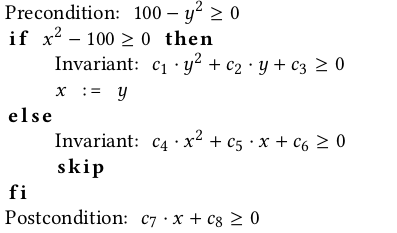
\includegraphics[scale=.55]{example1.png}
\end{center}
\end{frame}

\begin{frame}{Example}
    
    \begin{center}
    \includegraphics[scale=.55]{example1exec.png}
\end{center}
\end{frame}

\begin{frame}{Example}
    \begin{center}
    \includegraphics[scale=.55]{example1exec2.png}\end{center}
\end{frame}


\begin{frame}{Structural Operational Semantics: Basic Definitions}
    \begin{itemize}
        \item An infinite set of locations $\mathbf{Loc}$: $\xi \in \mathbf{Loc}$.
        \item A set of states $\mathbf{State}$: $\sigma \in \mathbf{State} = \mathbf{Var_*\rightarrow (Z + Loc +} \{\diamond\})$
        \item A set of heaps $\mathbf{Heap}$: $\mathcal{H} \in \mathbf{Heap} = (\mathbf{Loc}\times \mathbf{Sel}) \rightarrow_{fin} \mathbf{(Z + Loc +} \{\diamond\}) $
    \end{itemize}
    where the partial means not all selector fields need to be defined.
    
    The semantic of pointer arithmetic is given by:
        \begin{center}
        \includegraphics[scale=.55]{form1.PNG}
        \includegraphics[scale=.55]{form1def.PNG}
\end{center}
\end{frame}

\begin{frame}{Example}
    \begin{center}
        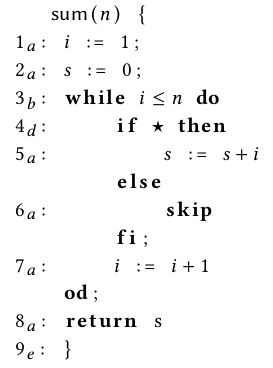
\includegraphics[scale=.55]{example2.PNG}
\end{center}
\begin{itemize}
    \item 
oval nodes: heap cells
\item 
$\xi_i$s': locations
\item labelled edges: heap
\item unlabelled edges: state
\end{itemize}

\end{frame}
\begin{frame}{Semantics of Expressions}
    Extend the old semantic to store and heap:
    \begin{center}
        \includegraphics[scale=.55]{form3.PNG}
        \includegraphics[scale=.55]{form4.PNG}
        \includegraphics[scale=.55]{form5.PNG}
\end{center}
\end{frame}

\begin{frame}{Semantics of Statements}

\begin{itemize}
    \item  $\langle [x:= a]^{\mathcal{l}}, \sigma, \mathcal{H}\rangle$
    \begin{center}
        \includegraphics[scale=.55]{form6.PNG}
\end{center}
    \item $\langle [x.sel := a]^{\mathcal{l}}, \sigma, \mathcal{H}\rangle$
    \begin{center}
        \includegraphics[scale=.55]{form7.PNG}
\end{center}
    \item \texttt{malloc}: allocation for pointers.
    \begin{center}
        \includegraphics[scale=.55]{form8.PNG}
\end{center}
\end{itemize}
\end{frame}
\begin{frame}{Semantic of Statements}
    For \texttt{malloc}: a limited reused strategy is used.
    \begin{itemize}
        \item $x$ can be reused: $[\texttt{malloc} x]^1; [x := \texttt{nil}]^2; [\texttt{malloc} x]^3$
        
        \item $x$ cannot be reused although unreachable: $[\texttt{malloc} x]^1; [x.cdr := \texttt{nil}]^2; [x := \texttt{nil}]^3; [\texttt{malloc} x]^4$
    \end{itemize}
\end{frame}

\begin{frame}{Shape Graphs: Abstraction of the Memory Configurations}
    \begin{definition}{Shape Graph}
        A shape graph is a triplet $(\texttt{S}, \texttt{H}, \texttt{is})$, where
        \begin{itemize}
            \item Abstract state $\texttt{S}$ is a map from variables to \emph{abstract locations}: 
            \[\texttt{S}\in \mathbf{AState} = \mathcal{P}\mathbf{(Var_*\times ALoc)}\]
            
            \item Abstract heap $\texttt{H}$ is set specifies the links between abstract locations : 
            \[\texttt{H}\in \mathbf{AHeap} = \mathcal{P}\mathbf{(ALoc \times Sel\times ALoc)}\]
            
            \item A set of abstract locations that are shared: 
            \[\texttt{is} \in \mathbf{IsShared} = \mathcal{P}\mathbf{(ALoc)}\]
        \end{itemize}
    \end{definition}
\end{frame}

\begin{frame}{Abstract Locations}
    The abstract locations have the form $n_X$ where $X$ is a subset of the variables of $\mathbf{Var}_*$:
    
    \[\mathbf{ALoc} = \{n_X\mid X\subseteq \mathbf{Var}_*\}\]
    
    Finiteness: the set $\mathbf{Var}_*$ is finite.
\begin{itemize}
    \item 
    Intuitively, $n_X$ is the abstraction of the location $\sigma(x)$ of pointer variables  $x \in X$
    \item We shall enforce: 
    
    \textbf{Invariant 1: } If $n_X$ and $n_Y$ occur in the same shape graph, then either $X = Y$ or $X \cap Y = \emptyset$.
    \item We use \emph{abstract summary location} $n_\emptyset $ to represent all locations that cannot be reached directly from the state without using the heap. 
\end{itemize}
\end{frame}

\begin{frame}{Example of Abstract Locations}
\begin{center}
        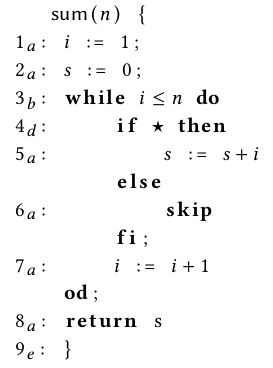
\includegraphics[scale=.67]{example2.PNG}
\end{center}

    
\end{frame}

\begin{frame}{Abstract States and Heaps}
\begin{itemize}
    \item Abstract state:
    Abstract state $\texttt{S}$ is a map from variables to \emph{abstract locations}: 
            \[\texttt{S}\in \mathbf{AState} = \mathcal{P}\mathbf{(Var_*\times ALoc)}\]
            
    \textbf{Invariant 2.} If $x$ is mapped to $n_X$ by the abstract state then $x\in X$.
    \vspace{1em}
    
    Define the set $ALoc(\texttt{S}) = \{n_X\mid \exists x : (x, n_X)\in \texttt{S}\}$ to be the abstract locations occuring in $\texttt{S}$.
    
    
    \item Abstract heap:  heap $\texttt{H}$ is set specifies the links between abstract locations : 
            \[\texttt{H}\in \mathbf{AHeap} = \mathcal{P}\mathbf{(ALoc \times Sel\times ALoc)}\]
            
    Intuitively, if $\mathcal{H}(\xi_1, sel) = \xi_2 $ and $\xi_1, \xi_2$ are represented by $n_V, n_V$ resp., then $(n_V, sel, n_W)\in \texttt{H}$.
    
      \vspace{1em}
    \textbf{Invariant 3.} Whenever $(n_V, sel, n_W)$ and $(n_V, sel, n_{W'})$ are in the abstract heap, then either $V = \emptyset$ or $W = W'$.
\end{itemize}
Both abstract state and abstract heap are changing along the execution.
\end{frame}

\begin{frame}{Example of Abstract States and Heaps}
    \begin{center}
        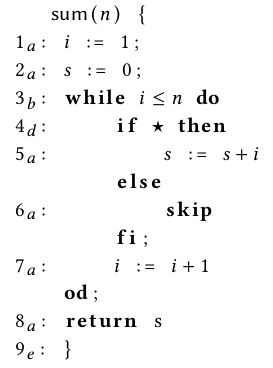
\includegraphics[scale=.67]{example2.PNG}\end{center}
\end{frame}

\begin{frame}{Sharing Information}
    A set of abstract locations that are shared due to pointers in the \emph{heap}: 
            \[\texttt{is} \in \mathbf{IsShared} = \mathcal{P}\mathbf{(ALoc)}\]
    \begin{center}
        \includegraphics[scale=0.4]{sharing.PNG}
    \end{center}
            
\end{frame}

\begin{frame}{Sharing Information}
    With above observations we have following invariant:
    \begin{center}
        \includegraphics[scale=0.55]{inv4.PNG}
    \end{center}
    
    And the connection of \texttt{is} to the abstract heap \texttt{H}:
    \begin{center}
        \includegraphics[scale=0.55]{inv5.PNG}
    \end{center}
    
    Sharing information clearly gives extra information: $n_\emptyset$
\end{frame}

\begin{frame}{Use of Shape Graph}

    \begin{center}
        \includegraphics[scale=0.55]{exec.PNG}
    \end{center}

\end{frame}

\begin{frame}{The Complete Lattice of Shape Graph}
\begin{align*}
            \texttt{S}\in \mathbf{AState} &= \mathcal{P}\mathbf{(Var_*\times ALoc)}\\
            \texttt{H}\in \mathbf{AHeap} &= \mathcal{P}\mathbf{(ALoc \times Sel\times ALoc)}\\
            \texttt{is} \in \mathbf{IsShared} &= \mathcal{P}\mathbf{(ALoc)}\\
\end{align*}
$\mathbf{ALoc} = \{n_Z\mid Z \subseteq \mathbf{Var}_*\}$. 

A shape graph $(\texttt{S,H,is})$ is compatible if it satisfies \textbf{Invariant 1.- 5.}, the set of compatible shape graphs is denoted:
\[\mathbf{SG} = \{(\texttt{S,H,is}) \mid \texttt{S,H,is} is compatible\}\]

The analysis will operate over on $\mathcal{P}(\mathbf{SG})$. Since it is a power set, it is trivially a complete lattice over union and subset relation. Due to the finiteness of $\mathbf{Var}_*$ is finite.
\end{frame}

\begin{frame}{The Analysis: Basic Framework}
    An instance of monotone framework: let $\mathcal{P}(\mathbf{SG})$ be the complete lattice of properties.
    
    For label consistent program $S_*$, we obtain a set of equations by
    \begin{center}
        \includegraphics[scale=0.55]{equations.PNG}
    \end{center}
    
    In the following, the transfer functions over different statements will be developed.
    
    The transfer function associate with label $l$: $f_{\mathcal{l}}^{\texttt{SA}}: \mathcal{P}(\mathbf{SG})\rightarrow\mathcal{P}(\mathbf{SG})$.
    
    \[f_{\mathcal{l}}^{\texttt{SA}}(SG) = \bigcup\{\phi_{\mathcal{l}}^{\texttt{SA}}((\texttt{S,H,is}))\mid (\texttt{S,H,is}) \in SG\}\]
    
    $\phi_{\mathcal{l}}^{\texttt{SA}}: \mathbf{SG} \rightarrow \mathcal{P}(\mathbf{SG})$.
\end{frame}
\begin{frame}{Transfer Functions}
\begin{itemize}
    \item 
    For $[b]^{\mathcal{l}}$ and $[\texttt{skip}]^{\mathcal{l}}$: $\phi_{\mathcal{l}}^{\texttt{SA}}((\texttt{S,H,is})) = \{(\texttt{S,H,is})\}$ 
    \item For $[x := a]^{\mathcal{l}}$ where $a$ is of the form $n, a_1 op_a a_2$ or \texttt{nil}:
    \begin{itemize}
        \item Renaming of abstract locations to exclude $x$: $k_x(n_Z) = n_{Z\backslash\{ x\}}$
        \item Function $\phi_{\mathcal{l}}^\texttt{SA}$ is given by
    \begin{center}
        \includegraphics[scale=0.55]{transfer1.PNG}
    \end{center}
    \end{itemize}
\end{itemize}
\end{frame}

\begin{frame}{Example}
    
    \begin{center}
        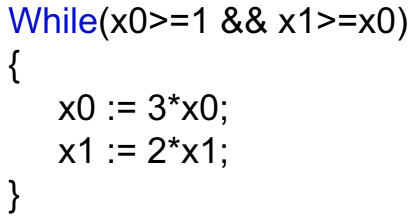
\includegraphics[scale=0.55]{example3.PNG}
    \end{center}
\end{frame}

\begin{frame}{Transfer Functions}
    \begin{itemize}
        \item For $[x := y]^{\mathcal{l}}$: - $x = y$. - $x \ne y$
        \item Based on previous $(\texttt{S}', \texttt{H}', \texttt{is}')$:
        
    \begin{center}
        \includegraphics[scale=0.55]{transfer2.PNG}
    \end{center}
    \end{itemize}
    Here $(y', n_Y)$ means $n_Y$ must can be visit by a pointer variable by state.
\end{frame}
\begin{frame}{Example}

    \begin{center}
        \includegraphics[scale=0.4]{example4.PNG}
    \end{center}

    
\end{frame}

\begin{frame}{Transfer Functions}
\begin{itemize}
    \item For $[x := y.sel]^{\mathcal{l}}$, we can regard it as an equivalent sequence:
    \[[t:=y.sel]^{l_1};[x := t]^{l_2};[t := nil]^{l_3}\]
    and 
    \[{f_{\mathcal{l}}^\texttt{SA}} = {f_{\mathcal{l_3}}^\texttt{SA} \cdot f_{\mathcal{l_2}}^\texttt{SA} \cdot f_{\mathcal{l_3}}^\texttt{SA}}\]
\end{itemize}
\end{frame}
\end{document}